\documentclass{beamer}
\usetheme{Antibes}

\usepackage[slovak]{babel}
\usepackage[utf8]{inputenc}

\begin{document}

\title{Advanced lighting in 2D graphics}
\author{Ferdinand Majerech}
\institute[UPJŠ]{Univerzita Pavla Jozefa Šafárika v Košiciach\\UPJŠ}

\begin{frame}[plain] 
  \titlepage
\end{frame}


\begin{frame}\frametitle{Intro}

\begin{itemize}
\item
  Attempting to create 2D lighing that "looks 3D"
\item
  Utilizing today's hardware advancements
\item
  Making it reusable for other projects
\item
  Author: Ferdinand Majerech
\item
  Supervisor: RNDr. Ladislav Mikeš
\end{itemize}

\end{frame}

\begin{frame}\frametitle{2D is not (completely) dead}

\begin{itemize}
\item
  Integrated, mobile GPUs
\item
  Easy programming
\item
  Art not limited by tech
\item
  Artists can ``cheat''
\item
  Don't always need 3D (RTS, Infinity-style RPG)
\end{itemize}

\end{frame}

\begin{frame}\frametitle{Pre-rendered graphics}

\begin{itemize}
\item
  3D -\textgreater{} tool -\textgreater{} 2D -\textgreater{}
  postprocessing -\textgreater{} game
\item
  Can look photorealistic
\item
  Low HW requirements
\item
  Lighting usually pre-rendered, static
\end{itemize}

\begin{center}
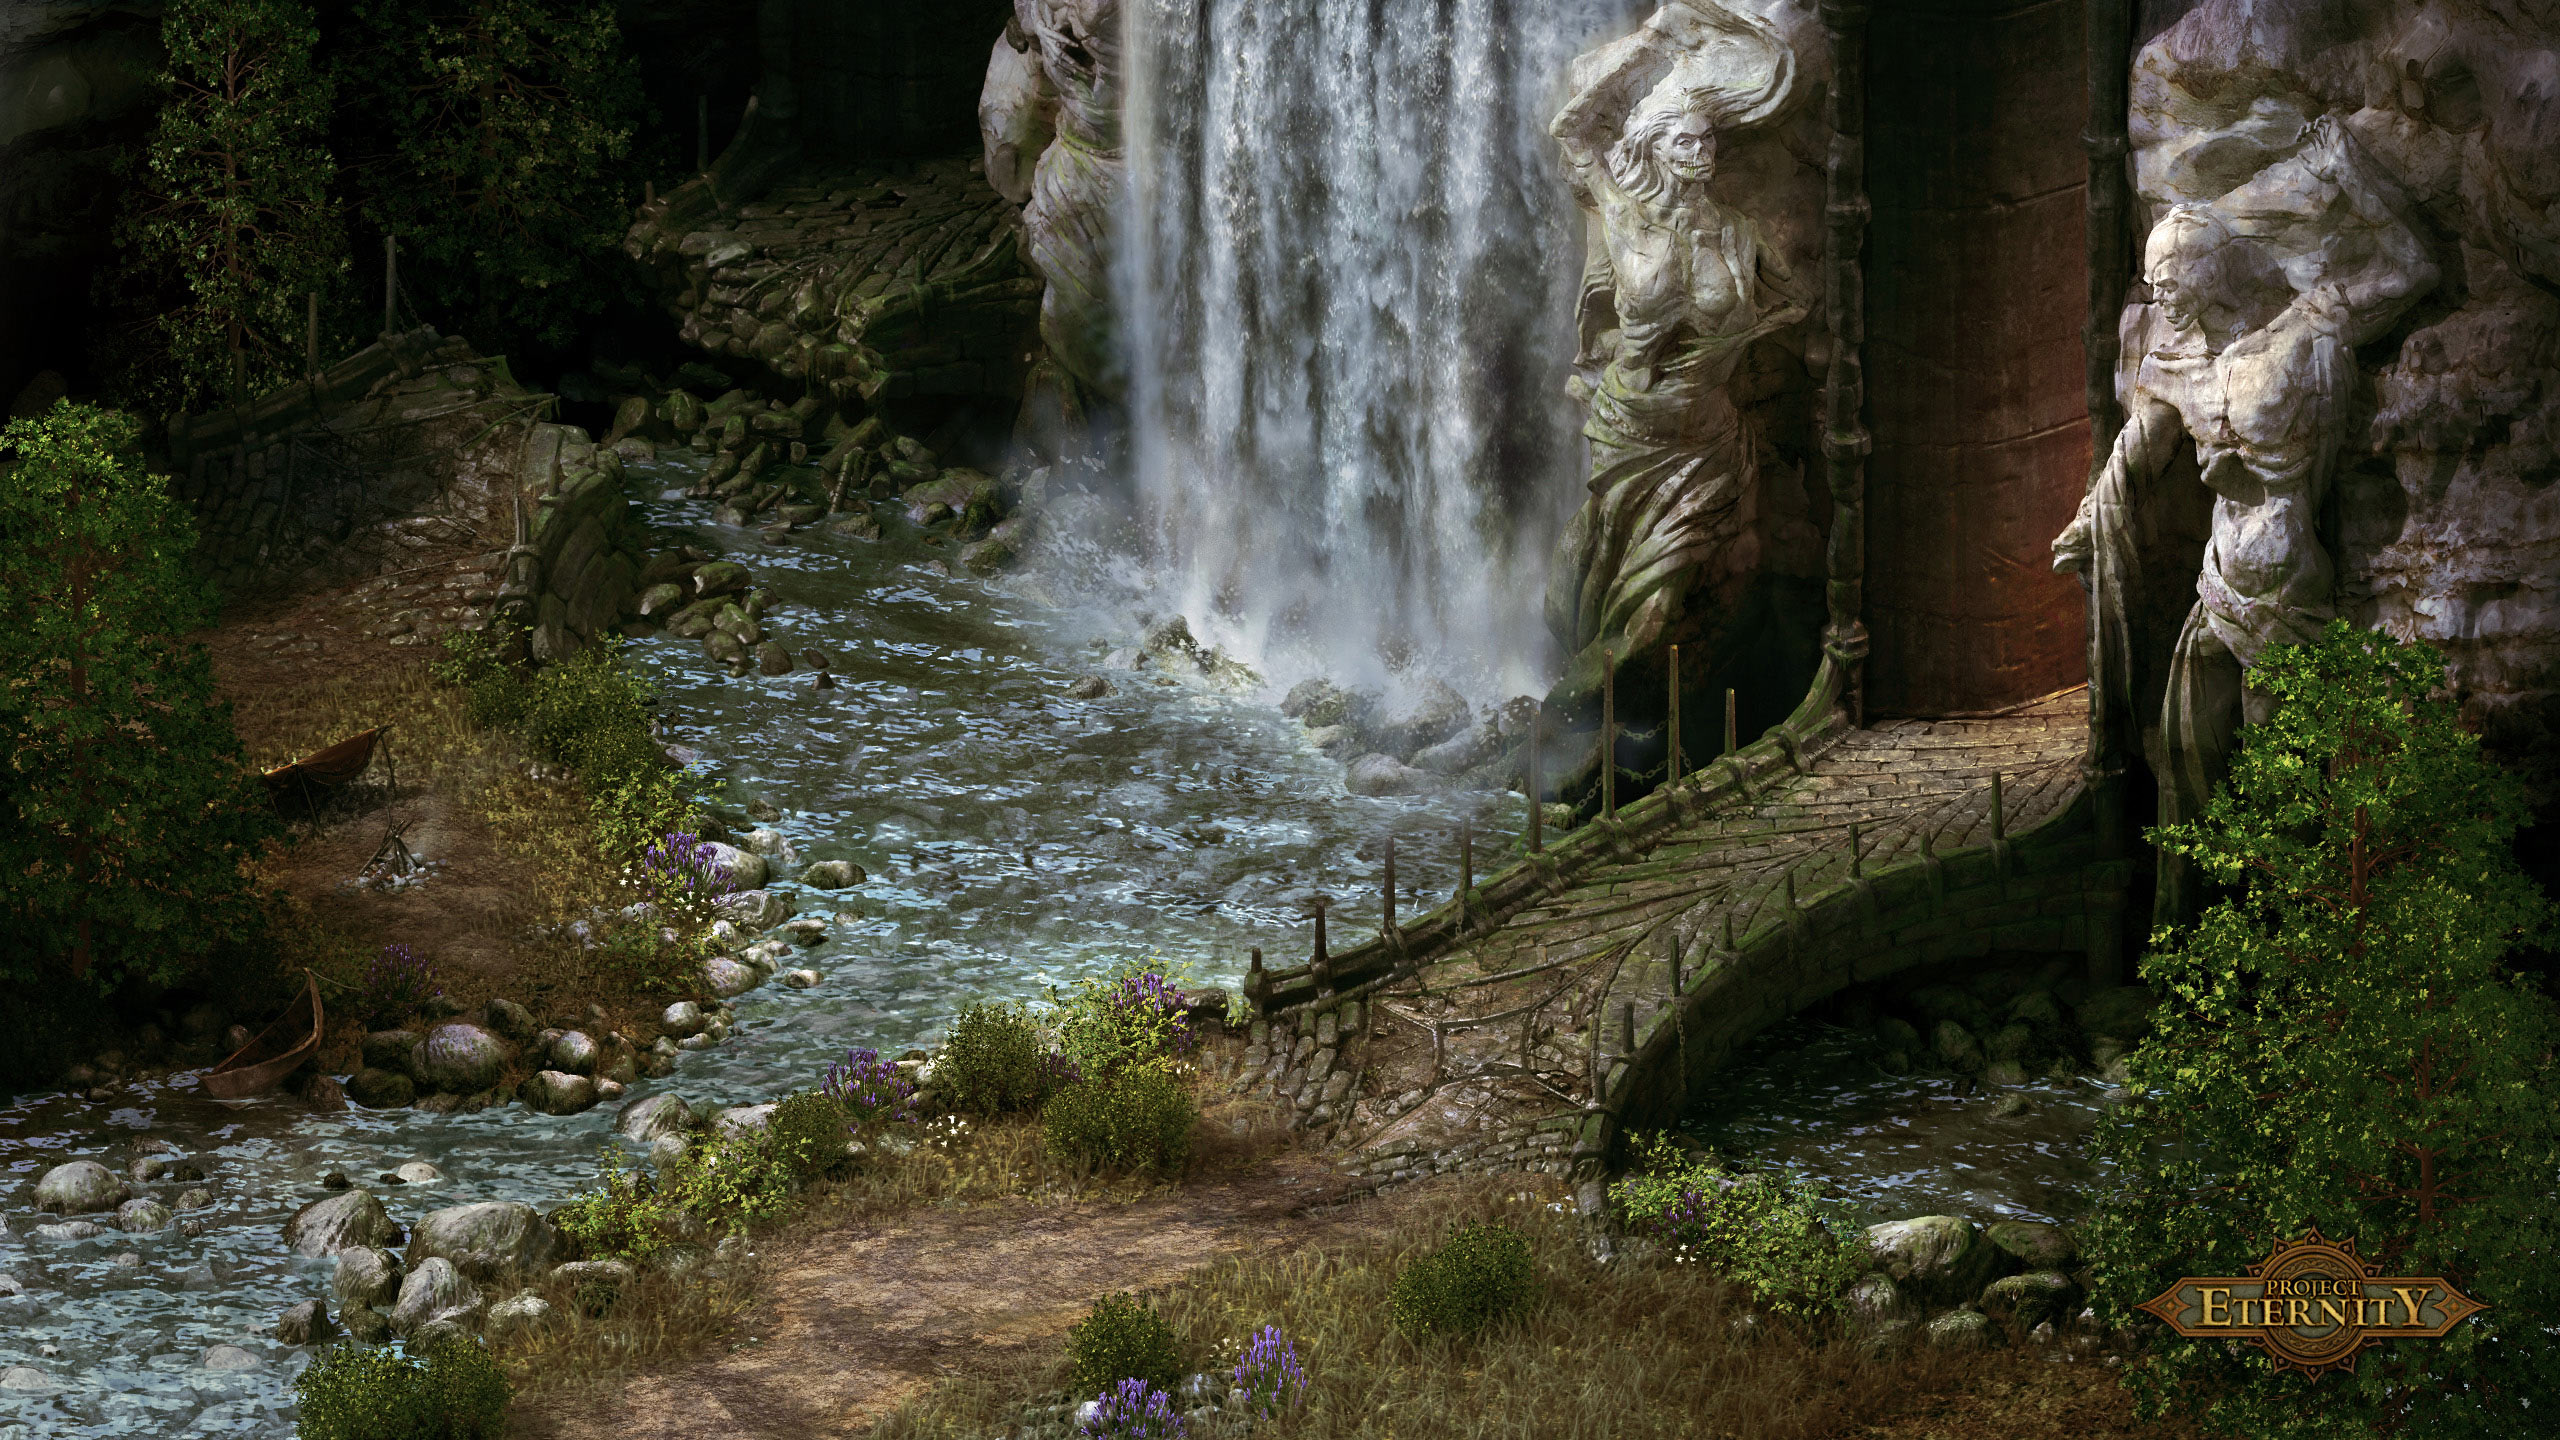
\includegraphics[width=0.75\textwidth]{eternity.jpg}
\end{center}

\end{frame}

\begin{frame}\frametitle{2D dynamic lighting in games}

\begin{itemize}
\item
  Homogenous lighting in a circle around the source
\item
  Shadowing in special cases (e.g. interior with vertical walls)
\item
  Can't light a complex object (no idea where ``front'' is)
\end{itemize}

\end{frame}

\begin{frame}\frametitle{We can do better}

\begin{itemize}
\item
  Not much progress since 2000
\item
  Generic Android phone has a better GPU than a GeForce 2
\item
  Fixed function GPUs are dead
\item
  We can build our software renderer in shaders
\end{itemize}

\end{frame}

\begin{frame}\frametitle{Goals}

\begin{itemize}
\item
  Move forward from 2000
\item
  Achieve ``real'' dynamic lighting in 2D
\item
  Make it easy to implement in any engine

  \begin{itemize}
  \item
    Tools
  \item
    Documentation
  \end{itemize}
\end{itemize}

\end{frame}

\begin{frame}\frametitle{Sources}

\begin{itemize}
\item
  Inspiration: Normal/Parallax/Relief mapping in 3D
\item
  Literature:

  \begin{itemize}
  \item
    B. T. Phong, Illumination for computer generated pictures,
    Communications of ACM 18 (1975), no. 6, 311--317.
  \item
    Blinn, J. F. 1978. Simulation of wrinkled surfaces. SIGGRAPH 1978.
  \end{itemize}
\item
  Cool stuff I want to use (time):

  \begin{itemize}
  \item
    Mitchell, J., McTaggart, G., and Green, C. 2006. Shading in Valve's
    source engine. SIGGRAPH 2006.
  \item
    Green, C. 2007. Efficient Self-Shadowed Radiosity Normal Mapping.
    SIGGRAPH 2007.
  \end{itemize}
\end{itemize}

\end{frame}

\begin{frame}\frametitle{Phong reflection model}

\begin{itemize}
\item
  Not Phong \emph{shading} model
\item
  Common in real-time 3D (fast \& good image)
\item
  Ambient, diffuse, specular
\item
  Resulting light: \raisebox{-1.8ex}{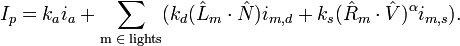
\includegraphics[scale=0.45]{phong1.png}}
\item
  Where R (reflection) is: \raisebox{-0.4ex}{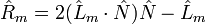
\includegraphics[scale=0.45]{phong2.png}}
\end{itemize}

\begin{center}
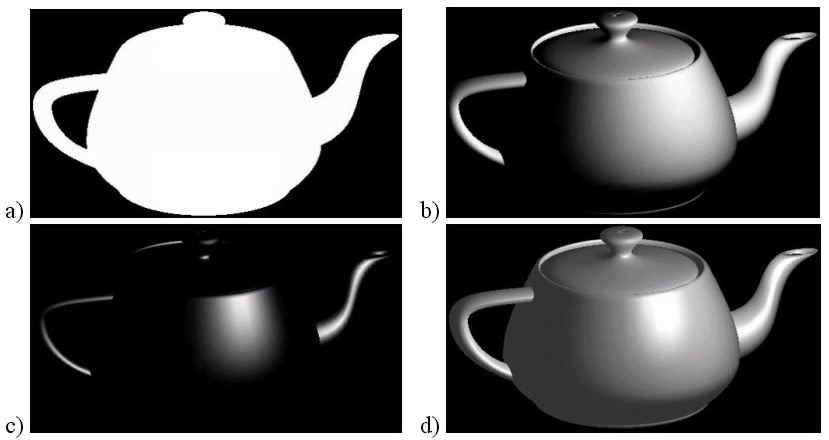
\includegraphics[width=0.6\textwidth]{ads.jpg}
\end{center}

\end{frame}

\begin{frame}\frametitle{Graphics pipeline}

\begin{itemize}
\item
  Vertex shader (3D primitives)

  \begin{itemize}
  \item
    Vertex positions, colors, etc.
  \item
    Not important here
  \end{itemize}
\item
  Fragment shader (pixels or subpixels)

  \begin{itemize}
  \item
    Textures
  \item
    Data calculated by vertex shader
  \end{itemize}
\end{itemize}
\begin{center}
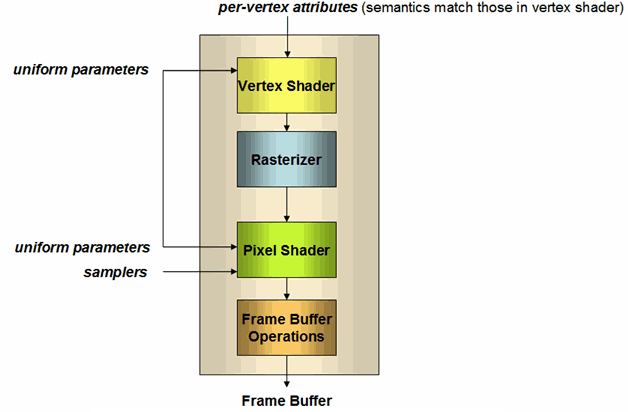
\includegraphics[width=0.45\textwidth]{pipeline.png}
\end{center}

\end{frame}

\begin{frame}\frametitle{Current approach}

\begin{itemize}
\item
  Phong reflection model ``in 2D''
\item
  Can be built upon later

  \begin{itemize}
  \item
    Self-shadowed radiosity normal mapping\ldots{} in 2D
  \item
    Environment mapping (sky reflection on shiny surfaces)
  \item
    \ldots{}
  \end{itemize}
\item
  Game simulation still needs to be 3D, but not graphics
\end{itemize}

\end{frame}

\begin{frame}\frametitle{Phong 2D}

\begin{itemize}
\item
  We only have 2D data (textures)
\item
  Need all data for Phong model

  \begin{itemize}
  \item
    From 3D simulation: Light/s, viewer positions
  \item
    From textures (per pixel):

    \begin{itemize}
    \item
      Relative position
    \item
      Normal
    \item
      Color (diffuse, specular)
    \end{itemize}
  \end{itemize}
\end{itemize}

\end{frame}

\begin{frame}\frametitle{Texture data}

\begin{itemize}
\item
  Normals (RGB8, RG8, palette)
\item
  Specular? (RGB8, G8)
\item
  Diffuse (RGBA8)
\item
  Position (RGB8, heightmap)
\item
  Memory/compute tradeoff
\item
  Anywhere between 40bpp and 104bpp is possible

  \begin{itemize}
  \item
    2000: 8bpp or 32bpp
  \item
    We have more VRAM now (but mobile\ldots{})
  \end{itemize}
\end{itemize}
\begin{center}
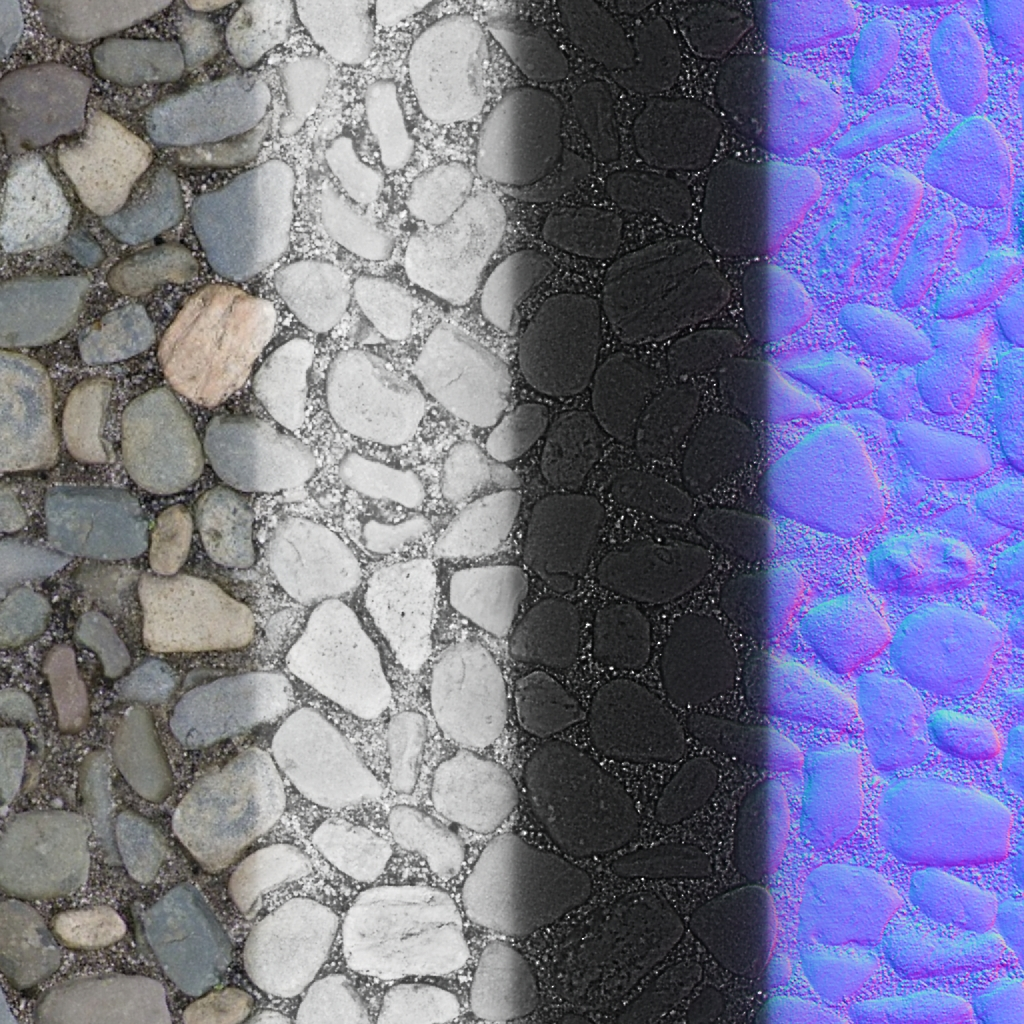
\includegraphics[width=0.3\textwidth]{maps.jpg}
\end{center}

\end{frame}

\begin{frame}\frametitle{Texture (sprite) authoring}

\begin{itemize}
\item
  Manual

  \begin{itemize}
  \item
    Hard
  \item
    Seriously? Paint positions in Photoshop?
  \end{itemize}
\item
  Pre-rendered

  \begin{itemize}
  \item
    No need to optimize models for a game
  \item
    Million triangles is not a problem
  \item
    Procedural textures
  \end{itemize}
\end{itemize}

\end{frame}

\begin{frame}\frametitle{Pre-rendering}

\begin{itemize}
\item
  Render-to-texture
\item
  Performance doesn't matter
\item
  Phong model (without the ``Phong'' part)
\item
  Render per-pixel data Phong model would use
\item
  For diffuse, a raytracer with AA is better
\item
  AA and vectors don't mix (2x resolution?)
\end{itemize}

\end{frame}

\begin{frame}\frametitle{Current status}

\begin{itemize}
\item
  Demo app not yet started
\item
  Working on pre-rendering

  \begin{itemize}
  \item
    Only loading models works (DerelictAssimp)
  \end{itemize}
\item
  Portable ``graphics engine'' complete

  \begin{itemize}
  \item
    VBuffers
  \item
    IBuffers
  \item
    Textures
  \item
    \textbf{Modular shaders}
  \item
    VFS, YAML, etc. (reused)
  \end{itemize}
\end{itemize}

\end{frame}

\begin{frame}\frametitle{Modular shaders}

\begin{itemize}
\item
  Can exchange shader program modules at run-time
\item
  Primitive polymorphism
\item
  Completely irrelevant to the work
\item
  Makes implementation much easier
\end{itemize}

\end{frame}

\begin{frame}\frametitle{Roadmap}

\begin{itemize}
\item
  Finish pre-rendering tool
\item
  Implement demo \& start working on the thesis
\item
  Time-based:

  \begin{itemize}
  \item
    GUI for the pre-rendering tool
  \item
    Improve the lighting model (esp. self-shadowing)
  \end{itemize}
\item
  Integrate into engine
\end{itemize}

\end{frame}

\begin{frame}\frametitle{More info}

\begin{itemize}
\item
  \href{http://kiithcoding.nfshost.com}{http://kiithcoding.nfshost.com}
\item
  \href{https://github.com/kiith-sa/awesome2D}{https://github.com/kiith-sa/awesome2D}
\item
  D
\item
  OpenGL2/GLSL
\item
  Assimp
\item
  SDL2
\end{itemize}

\end{frame}

\begin{frame}\frametitle{Thank you for your attention!}

\end{frame}

\end{document}
